\chapter{Introduction}
\label{Chapter1}
This chapter is devoted to the introduction of the Swampland program, starting from the basic background of the effective field theories, which is indispensable to the Swampland program, then what the Swampland is, and the Swampland conjectures, putting stresses mainly on the Swampland distance conjectures, which is going to be center of the discussion later. 
\section{Effective Field Theory}
Before jumping into the concepts of the Swampland, let us take a brief introduction to the effective field theory, since the Swampland program is interested in the conditions where some low energy EFT with gravity can always be a consistent theory at some higher energy scale (UV theory). Therefore, there is no doubt that it is necessary to have good knowledge of EFTs, and how they can deal with the energy scales, in order to proceed to the understanding of the Swampland program and its appications.    
%\parencite{agmon_lectures_2022}
\subsection{Basic Concept}
Comparing to the full theories, which are supposed to be valid up to arbitrarily high energy scales, the effective field theories (EFTs) describe the physical phenomena only below a certain energy scale $\Lambda$, while above this scale, EFTs are broken and to be modified. In this sense, for an experiment done with the energy scale of order $\Lambda$, any knowledge about physics at higher scales $\Lambda _{0} \gg \Lambda$ are not required, but only finite number of parameters whose values can be obtained from experiments are. This way, for instance in order to make a description of the particle collisions at LHC, what is required is only the theory with cut-off scale $\Lambda \sim 1\text{TeV}$, which is the effective theory for this case, without understanding of its full theory which describes the particles' behavior. This is one of the general bottom-up way to adopt the EFTs in situations such that the ful theory is unknown, and even not necessary. There is also a top-down usage where the full theory, or another EFT with higher cut-off scale, is known, and EFTs are used to simplify its computations by lowering the energy scale, such as QCD, a full theory for the strong interaction.  

%\subsection{Integrating out higher degrees of freedom}


\section{The Swampland Program}
As stated above, the Swampland program pursues the constraints that EFT has to obey to be consistent in the quantum gravity theory. Once gravity is taken into account, not every theory of quantume field theory would be consistent. In this section, only the Distance conjecture, its connection with other conjectures, and realization would be discussed with certain detail, while others are going to be given briefly for the purpose of this thesis. More profound introductions for them would be left for the references such as %\parencite{}.

\subsection{What is the Swampland?}
A starting point of the Swampland program is asking a question whether some quantum EFT coupled with Einstein gravity always can be back to UV theory with cpnsistency, that is,it can be UV completed or not. And the answer is no. Not every EFT cannot be UV completed so that it is consistent with QG. Then the next question to be considered is: under what conditions an EFT is so? More formaly, the Swampland program aims to identify certain criteria to determine if the EFT can be coupled to gravity at higher energy scales. Such constraints are called \emph{swampland constraints}. Then here comes a definition of the Swampland as follows:
\begin{tcolorbox}[title=The Swampland,
    title filled=false,
    colback=blue!5!white,
    colframe=blue!75!black]
    The low-energy EFT that cannot be UV completed in the consideration of quantum gravity.  %\textbf{tcolorbox}.
\end{tcolorbox} 
Therefore, it is equivalent to say that an EFT does not satisfy the Swampland constraints, in other words, it is not UV consistent theory of quantum gravity, if it is in the Swampland. On the other hand, the EFTs fulfill those conditions are named \emph{Landscape}. So in those languages, the ultimate goal the Swampland program is trying to achieve is to specify what separates the Swampland and the landscape. \\
\indent Notice that those constraints are supposed to vanish as the gravity is decoupled, i.e. the Planck mass $M_{p}$ is sent to infinity, in order for them to be the Swampland constraints. This observation is followed by the fact that the higher the energy scale above which the EFT breaks down is, the more strict the constraints are. It is shown in figure \ref{fig:swampland}, where cone drawn in blue stands for the landscape, surrounded by the Swampland. The Swampland constraints become stronger as the energy scales increase and eventually one may get closer to the QG scale as depceted by the blue cone. \\ 
\tdplotsetmaincoords{80}{100}

\begin{figure}
\begin{tikzpicture}[scale=4,tdplot_main_coords]


\draw[thick,->] (0,0,0) -- (1,0,0) node[anchor=north east]{Theory Space};
\draw[thick,->] (0,0,0) -- (0,1,0) node[anchor=north west]{Theory Space};
\draw[thick,->] (0,0,0) -- (0,0,1) node[anchor=south]{Energy Scale};

\draw(0.5,0.5,0) circle (0.45) node[below = 9pt] {Swampland};
\shadedraw[blue](0.6,0.6,0) circle (0.1);
\draw[blue,thick](0.62,0.5,0) parabola (0.6,0.6,0.9);
\draw[blue,thick](0.6,0.705,0) parabola (0.6,0.6,0.9) node[above = 1pt] {Quantum Gravity};
\draw[->] (1.2,1.2,0) node[below] {Landscape} --  (0.61,0.68,0);
\end{tikzpicture}
\caption{EFTs on the theory space. There is a landscape inside the Swampland of EFTs. Since the constraints get more strict at the higher energy scale, the space consistent with QG forms a cone shape.}
\label{fig:swampland}
\end{figure}

\indent As repeatedly stated, there is a specific cut-off, say, $\Lambda$ above which the EFT is no longer valid. It is necessary for the EFT to be modified so that the new EFT is valid above the cut-off $\Lambda$ with some new cut-off $\Lambda'$ by integrating in new degrees of freedom, as opposed to integrating out when obtaining an EFT given some UV theory. However, this process cannot be proceeded indefinitely: no EFT cannot deal with infinitely many degrees of freedom. Therefore, any EFT has a certain cut-off where it cannot be modified anymore to obtain a consistent theory coupled to Einstein gravity. This leads to an important notion. An EFT is determined if it is on the Swampland or the landscape not only by whether it is possible to be UV completed in QG, but also by whether it is not broken down, that is, it is valid or not up to such a new cut-off. This fact can be seen from figure \ref{fig:swampland} and is shown more clearly in figure \ref{fig:cross}. Given an EFT belonging to the landscape at some lower energy scale, it belongs to the Swampland once the energy scale is greater than specific value. 

\begin{figure}
    \centering
    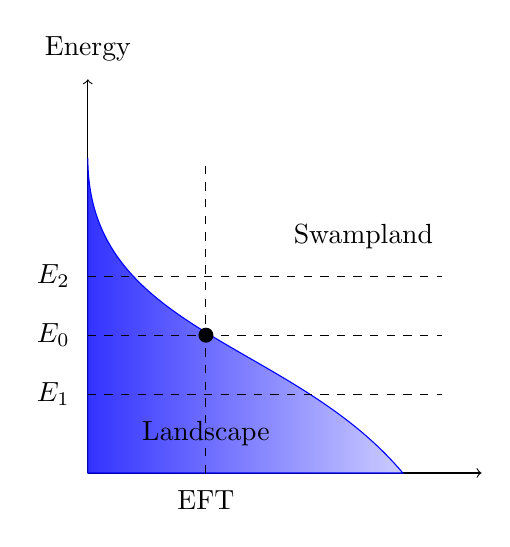
\begin{tikzpicture}[scale = 5]

        \draw[->] (0,0) -- (1,0);
        \draw[->] (0,0) -- (0,1) node[above=3pt]{Energy};
        \shadedraw[left color=blue!80!white,right color=blue!20!white, draw=blue] (0,0) -- (0,0.8) to [out=270, in=130] (0.8,0) -- cycle
        (0,0.2) node[left=3pt]{$E_{1}$}
        (0,0.5) node[left=3pt]{$E_{2}$}
        (0.3,0.1) node{Landscape}
        (0.7,0.6) node{Swampland};
        \draw[style=dashed] (0.3,0) node[below=3pt]{EFT} -- (0.3,0.8);
        \draw[style=dashed] (0,0.35) node[left=3pt]{$E_{0}$} -- (0.9,0.35);
        \draw[style=dashed] (0,0.2) -- (0.9,0.2);
        \draw[style=dashed] (0,0.5) -- (0.9,0.5);
        \filldraw[black](0.3,0.35) circle (0.5pt);
    \end{tikzpicture}
    \caption{This shows the cross section of figure \ref{fig:swampland}. Given an EFT at some lower energy scale, it belongs to the landscape as long as its characteristic energy is below $E_{0}$. However, the same EFT turns to be in the Swampland if the energy scale is above it. For instance, this EFT is in the landscape if it provides a description of physics of energy $E_{1}$, while it is in the Swampland if it does of $E_{2}$.}
    \label{fig:cross}
\end{figure}
Thus, whether an EFT belongs to the Swampland or the landscape is determined by at which energy scale it is used for an illustration of a physical system. As such energy increases, there are more strict constraints, and eventually the landscape gets smaller and smaller.

\subsection{Swampland Conjectures}
Those sonctraints are still investigated and not uderstood well yet. It is why they are called the Swampland conjectures, not being proven yet. However, they have been gradually accepted widely as sufficient amont of evidence to support them has been collected. Figure \ref{fig:connection} shows the conjectures and connections among them.
\begin{figure}
    \centering
    \begin{tikzpicture}
        \path[mindmap,concept color=black,text=white]
    node[concept] {No Global Symmetries}
    [clockwise from=0]
    child[concept color=green!50!black] {%
      node[concept](WG){Weak Gravity Conjecture}
      [clockwise from=0]
      child {node[concept] {Non-SUSY AdS Instability Conjecture} }
      %child {node[concept] {data structures} }
      %child {node[concept] {pro\-gramming languages} }
      %child {node[concept] {software engineer\-ing} }
    }  
    child[concept color=blue] {%
      node[concept](DC) {Swampland Distance Conjecture}
      [clockwise from=-30]
      child {node[concept] {No deSitter} }
      child {node[concept] {No Scale Separation in AdS} }
    }
    child[concept color=red] {node[concept] {Completeness Hypothesis} }
    child[concept color=orange] {node[concept] (TC){Trivial Cobordism} };
    \begin{pgfonlayer}{background}
        \draw [circle connection bar]
        (WG) edge (DC);
    \end{pgfonlayer}
    \end{tikzpicture}
    \caption{A schematic map of the Swampland conjectures}
    \label{fig:connection}
\end{figure}
In the following sections, only two conjectures will be discussed in detail, which are most relevant for the purpose of the thesis. The connestions between conjectures might indicate that some of them are equivalent statements with different appearances. Unifying them by better understanding of QG in the future is one of the goal of this area.

\subsection{No Global Symmetries in Quantum Gravity}
The absence of global symmetries is considered as the first Swampland conjecture, and widely accepted. The statement of the conjecture is as follows:
\begin{tcolorbox}[title=No Global Symmetries Conjecture,
    title filled=false,
    colback=blue!5!white,
    colframe=blue!75!black]
    There are no exact global symtries in quantum gravity.  %\textbf{tcolorbox}.
\end{tcolorbox} 
First of all, it is worth to recall briefly that a global symmetry is defined as an invariance under transformations described by a unitary operator commuting with the Hamiltonian. According to Noether's theorem, the continuous symmetry of a system indicates the existence of the conserved quantity, or charge, in it. For instance, the spatial translational symmetry leads to the conservation of momentum. In order to see illustrate what would make it invalid if a global symmetry is allowed in quantum gravity, assume that there \emph{IS} a continuous global symmetry with a conservation charge in quantum gravity. Suppose a black hole is charged by throwing a conserved charge into it under a $U(1)$ global symmetry, it will evaporate decreasing its mass but maintaining its charge because Hawking radiation contains same number of positive/negative charged particles. Letting it evaporate completely, charge is supposed to vanish. Thus, it leads to a violation of the charge conservation. Also, even if such evaporation stops , and ends up with a remnant of mass $M \sim M_{P}$, since, according to the No-hair theorem, stable black holes can be distinguished from outside only by its mass, angular momentum, and gauge charge, it is impossible to determine its global charge given a black hole of a specific mass. Therefore, the conservation gets invalid. Hence, there cannot be global symmetries in a theory of quantum gravity.This discussion can be extended to discrete symmetries and also to more generic global symmetries. Those are followed by the proposal of the Cobordism conjecture, which will be presented later. The arguments above are rather motivation that proofs to grasp good intuitions for the conjecture. There are more formal evidences mainly from string theory. Here most of discussions for such proofs is from %\parencite{}.
It is important to note that it is permitted that there is a low-energy theory with a global symmetry, as long as at higher energies such symmetry is gauged or broken. While it still gives understanding of the principles of quantum gravity, the No-global symmetries conjecture doesn't provide meaningful phenomenological constraints since nothing about at which scale such a global symmetry gets forbidden is stated. However, it is followed by other conjectures such as the Weak Gravity Conjectures and the Swampland Distance Conjecture, which give more concrete constraints, as expansions and refinements of the concept of the impossibility of exact global symmetries in quantum gravity. 
\subsection{Swampland Distance Conjecture}
The Swampland Distance Conjecture (SDC) is the one of the Swampland conjectures which give certain quantitative constraints. It provides a restriction on an EFT of quantum gravity when it is getting closer to where a global symmetry is restored. \\
\indent The motivation for the conjecture comes from the investigation in a moduli space, which is a space parametrized by the vacuum expectation value of some scalar fields. It is particular interest in that space to observe how an EFT changes as moving toward a certain direction where a global symmetry gradually, that is, some gauge coupling decreases to zero, because an exact global symmetry is not acceptable in quantum gravity. Therefore it is expected there is some phenomena in such limits in order to protect a theory to get back a global symmetry. One natural assumption to do so is that such poins are infinitely far away in a space. In addition, as an approximate global symmetry is getting exact as moving towards those limits, it is reasonable that an EFT is supposed to become an invalid description continuously. That is also predicted by the consequence of the Weak Gravity Conjecture. \\
\indent One important key point is that it is characteristic for a quantum gravity. Without considerring the quantum gravity, it is perfectly fine to have a point where a gauge coupling vanishes at infinite distance, and being close to it with maintaining a valid theory. Once the quantum gravity is taken into account, since taking a exact global symmetry strictly forbidden, an EFT should break down continuously as being closing to those limits. This can be generalized to other types of global symmetries. The Swampland Distance Conjecture provides information how EFT behaves when approaching infinite distance in a moduli space, and what features of quantum gravity makes it happen. \\
\indent Consider an EFT coupled to Einstein gravity with moduli space $\mathcal{M}$ parametrized by scalar fields, and whose metric $g_{ij}$ is given by its kintic term. The first statement of the conjecture is as follows: Starting from a point $P \in \mathcal{M}$, there always exits a point $Q \in \mathcal{M}$ at infinite geodesic distance $d(P,Q)$. The second part of the conjecture describes a phenomena supposed to happen as approaching a point at infinite field distance:
\begin{tcolorbox}[title=Swampland Distance Conjecture,
    title filled=false,
    colback=blue!5!white,
    colframe=blue!75!black]
    There happens an infinite tower of states which becomes exponentially light with the geodesic distance such as 
    \begin{align}
        M(Q) \sim M(P) e^{-\lambda d(P,Q)}
    \end{align}
    with $\lambda$ an $\order*{1}$ constant in Planck units. 
\end{tcolorbox}
It is abstractly illustrated in figure \ref{fig:tower}. Since an EFT cannot deal with infinitely many degrees of freedom under its cut-off, the emergence of the infinite tower of states indicates the breakdown of EFT. Thus, there supposed to be a quantum gravity cut-off associated to the infinite tower of states, which decreases exponentially with the geodesic distance:
\begin{align}
    \Lambda _{\text{QG}} = \Lambda e^{-\lambda d(P,Q)}
\end{align}
\begin{figure}
    %\centering
    \begin{subfigure}{.5\linewidth}
        %\centering
        \begin{tikzpicture}[scale=5]
            \draw[->] (0,0) -- (0,1) node[above=3pt]{M};
            \draw[style = dashed] (-0.4,0.8) node[left=3pt] {$\Lambda$} -- (0.4,0.8);
            \draw[-] (-0.03,0.1) -- (0.03,0.1);
            \draw[-] (-0.03,0.2) -- (0.03,0.2);
            \draw[-] (-0.03,0.3) -- (0.03,0.3);
            \draw[-] (-0.03,0.4) -- (0.03,0.4);
            \draw[-] (-0.03,0.5) -- (0.03,0.5);
            \draw[-] (-0.03,0.6) -- (0.03,0.6);
            \draw[-] (-0.03,0.7) -- (0.03,0.7);
            \draw[-] (-0.03,0.9) -- (0.03,0.9);
        \end{tikzpicture}
    \end{subfigure}
    \begin{subfigure}{.5\linewidth}
        %\centering
        \begin{tikzpicture}[scale=5]
            \draw[->] (0,0) -- (0,1) node[above=3pt]{M};
            \draw[style = dashed] (-0.4,0.8) node[left=3pt] {$\Lambda$} -- (0.4,0.8);
            \draw[-] (-0.03,0.1) -- (0.03,0.1);
            \draw[-] (-0.03,0.2) -- (0.03,0.2);
            \draw[-] (-0.03,0.3) -- (0.03,0.3);
            \draw[-] (-0.03,0.4) -- (0.03,0.4);
            \draw[-] (-0.03,0.5) -- (0.03,0.5);
            \draw[-] (-0.03,0.6) -- (0.03,0.6);
            \draw[-] (-0.03,0.7) -- (0.03,0.7);
            \draw[-] (-0.03,0.9) -- (0.03,0.9);
            \draw[-] (-0.03,0.65) -- (0.03,0.65);
            \draw[-] (-0.03,0.75) -- (0.03,0.75);
            \draw[-] (-0.03,0.55) -- (0.03,0.55);
            \draw[-] (-0.03,0.45) -- (0.03,0.45);
            \draw[-] (-0.03,0.35) -- (0.03,0.35);
            \draw[-] (-0.03,0.25) -- (0.03,0.25);
            \draw[-] (-0.03,0.15) -- (0.03,0.15);
            \draw[-] (-0.03,0.05) -- (0.03,0.05);
        \end{tikzpicture}
    \end{subfigure}
    \caption{Left picture represents an EFT with a cut-off $\Lambda$. There are finitely many states below this cut-off. As moving toward a point at infinite geodesic distance, it becomes as shown right. Continuously, the closer it is to such a point, the more degrees of freedom coming in the EFT description. After all, in order to try to avoid infinitely many degrees of freedom for an EFT, a cut-off is supposed to fall down to zero.}
    \label{fig:tower}
\end{figure}
\indent To gain an insight how SDC is realized, consider an example of a theory compactified on a circle of radius R. Through a Kaluza-Klein circle compactification in such a circle, its modes, KK modes, are known to have a mass as:
\begin{align}
    \label{eq:1.3}
    m_{n}^{2} = \frac{n^{2}}{R^{2}} ,& \qq{} n \in \mathbb{Z}. 
\end{align}
Taking this R to be the modulus controlling the radius of the circle, the kinetic term of the field R can be written in $\mathcal{L} _\text{{kin}} \sim \frac{1}{R^{2}} \partial_{M} R \partial ^{M} R$. The geodesic distance between two points, namely $R_{i}$ and $R_{f}$, in the field space is mesured by the metric, and yields to:
\begin{align}
    d(R_{i},R_{j}) = \abs \Big{\ln (R_{f} / R_{i})}
\end{align} 
From this, it is easy to see that there are two points which give an infinite proper distance starting from any finite radius, $R \to \infty$ and $R \to 0 $. The first limit gives a predicted behavior from eq. \ref{eq:1.3}. On the contrary, it seems that the SDC is violated for the limit $R \to 0$. However, considering the string theory, which has another infinite tower of states, winding states, whose masses given:
\begin{align}
    \label{eq:1.5}
    m_{w} ^2 = \frac{w^{2} R^{2}}{(\alpha ')^2}
\end{align}
where $\alpha '$ stands for the string length, and they also behave as expected. In this sense, there is a critical connection betweem the realization of SDC and the existence of T-duality. \\
\indent To sum up, the SDC can be thought of as a constraint on the validity for finite field variations, as an EFT at a point in moduli space cannot be extended to an arbitrary far point from initial one. By approaching such a point, an infinite number of degrees of freedom would become exponentially light and eventually an EFT description broken. So far computations for the distance ahve been considered on the moduli space. Nevertheless, this notion of the distance can be generalized to the one between more generic field with a generic metric given also by the kinetic term. It will be investigated how the renoemalization group affects on the statement of this conjecture later. 
\subsection{Other Conjectures}
